\section{METODOLOGI}

Penelitian ini dilaksanakan sesuai dengan blok diagram pada Gambar 3.1. Blok diagram tersebut
merupakan metodologi penelitian yang disusun sesuai dengan langkah-langkah yang dilakukan dalam penelitian ini.

\begin{figure} [ht] \centering
  \counterwithin{figure}{section}
  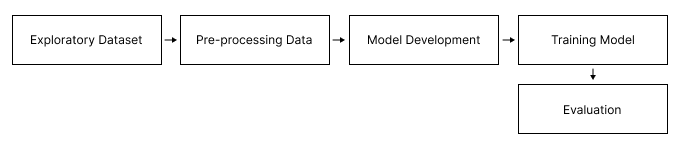
\includegraphics[width=160mm]{gambar/metodologi.png}
  \caption{Metodologi Penelitian}
\end{figure}


\subsection{Exploratory Dataset}
Melakukan analisa pada data untuk mendapatkan gambaran awal pada data. Analisa yang dilakukan yaitu
memeriksa informasi pada data (tipe data pada tiap data), memeriksa \emph{missing value} {(data yang hilang pada baris data)},
memeriksa duplikasi pada data.


\subsection{Pre-processing Data}
Pada proses ini dataset yang telah dilakukan analisa akan dilakukan pra-pemrosesan sebelum dataset dapat digunakan
untuk melakukan pelatihan pada model. Pada sistem rekomendasi pra-pemrosesan data yang biasa dilakukan seperti menghapus data
yang tidak diperlukan untuk proses pelatihan, menghapus \emph{missing value} jika ada, melakukan normalisasi pada data (biasanya mentransformasikan data kedalam range yang sama),
melakukan pembagian data pelatihan dan data percobaan.

\subsection{Training Model}
Melakukan pelatihan pada dataset menggunakan model \emph{Decision Tree}, untuk mendapatkan yang dapat memberikan rekomendasi
mata kuliah.

\subsection{Evaluation}
Evalusai dilakukan dengan melakukan rekomendasi pada data percobaan. Jika dirasa rekomendasi belum cukup baik. Maka perlu melakukan
\emph{tuning parameter} pada model seperti jumlah pohon yang digunakan pada model \emph{Decision Tree}, jumlah iterasi pelatihan dan
beberapa parameter lain sampai model dapat memberikan rekomendasi dengan cukup baik.

